\section*{Problem 2 - Underwater Vehicles}
Answer Problem 2 in this file. 
\subsection*{Problem 2.1}
Answer problem 2.1 here. The Greek letters for sideslip, crab and course are $\beta_r$, $\beta$ and $\chi$, respectively. The Greek letter for the flight-path angle is $\gamma$.

\subsection*{Problem 2.2}
Answer Problem 2.2 here. The body-fixed velocities can be written as
\begin{equation}
\label{eq:velocity}
	\begin{bmatrix}
		u \\
		v \\
		w
	\end{bmatrix}
	= 
	\begin{bmatrix}
		U \cos( \omega t)\\
		U \sin(\omega t)\\
		0	
	\end{bmatrix}
\end{equation}

\subsection*{Problem 2.3}
Answer Problem 2.3 here.

\subsection*{Problem 2.4}
Answer Problem 2.4 here. Figures can be inserted as:
\begin{figure}[ht]
	\centering
	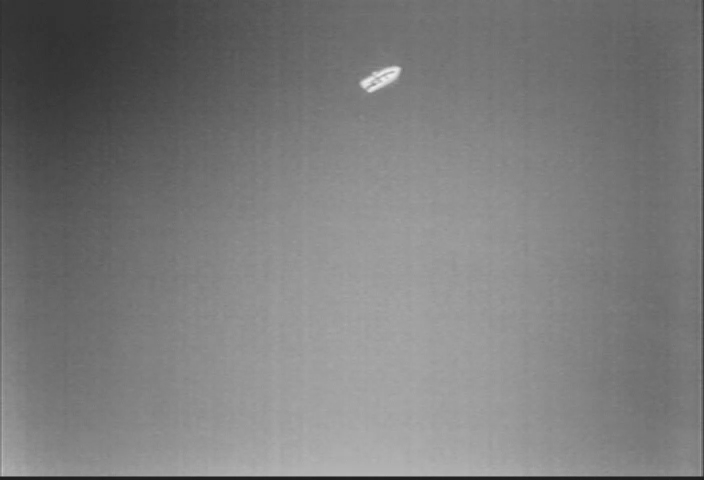
\includegraphics[width=0.7\textwidth]{assignment_1/rapport/figures/fig1} % Filename is "fig1.png" and must be located in the same folder as this file. If you have a folder containing all the figures you can use "Figures/fig 1" as long as the "Figures" folder is placed in the same folder as this file.
	\caption{Figure of something useful.}
	\label{fig:fig1}
\end{figure}

You can now refer to this figure as \figref{fig:fig1}. You can also insert figures side-by-side:
\begin{figure}[ht]
	\centering
	\begin{subfigure}[b]{0.45\textwidth}
		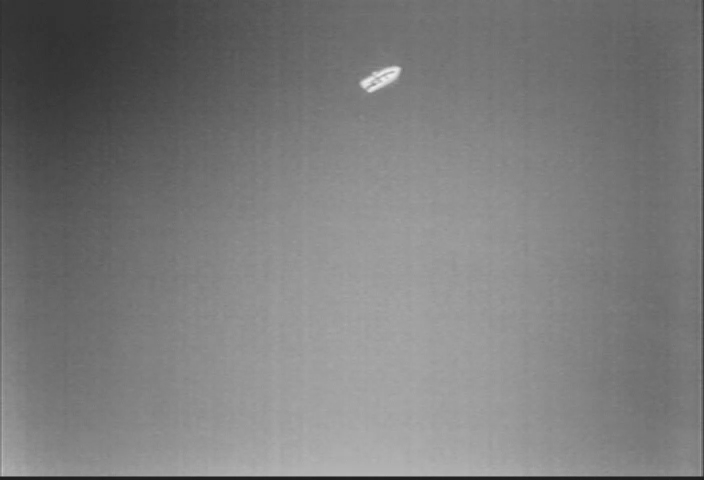
\includegraphics[width=\textwidth]{assignment_1/rapport/figures/fig1}
		\caption{caption..}
		\label{fig:2a}
	\end{subfigure}
	~ %add desired spacing between images, e. g. ~, \quad, \qquad, \hfill etc. 
	%(or a blank line to force the subfigure onto a new line)
	\begin{subfigure}[b]{0.45\textwidth}
		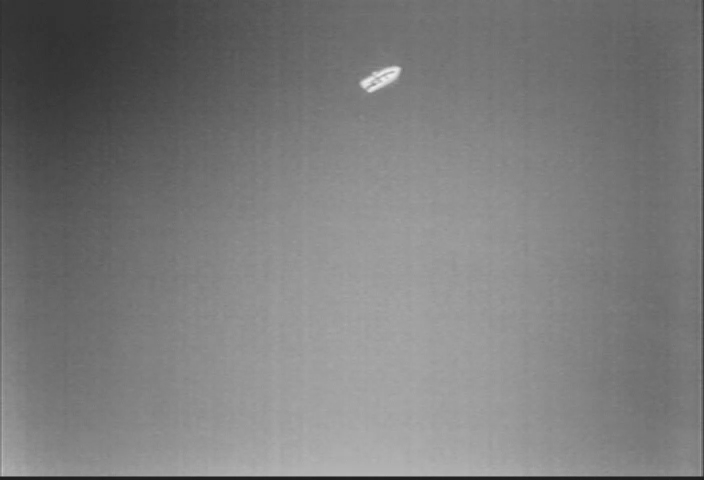
\includegraphics[width=\textwidth]{assignment_1/rapport/figures/fig1}
		\caption{caption..}
		\label{fig:2b}
	\end{subfigure}
	\begin{subfigure}[b]{0.45\textwidth}
		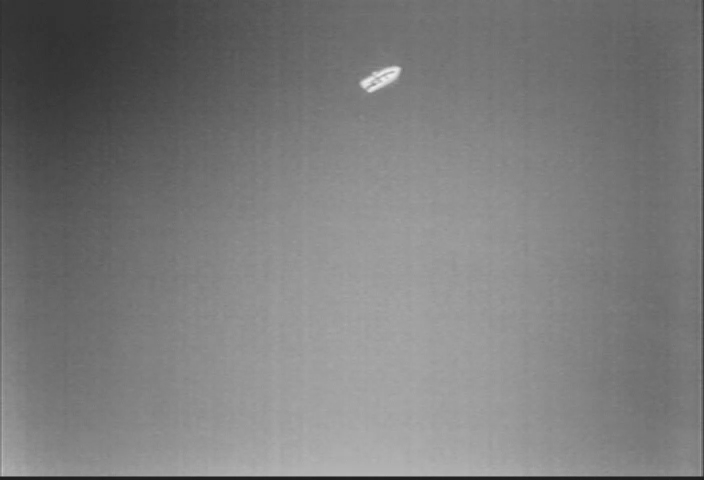
\includegraphics[width=\textwidth]{assignment_1/rapport/figures/fig1}
		\caption{caption..}
		\label{fig:2c}
	\end{subfigure}
	\begin{subfigure}[b]{0.45\textwidth}
		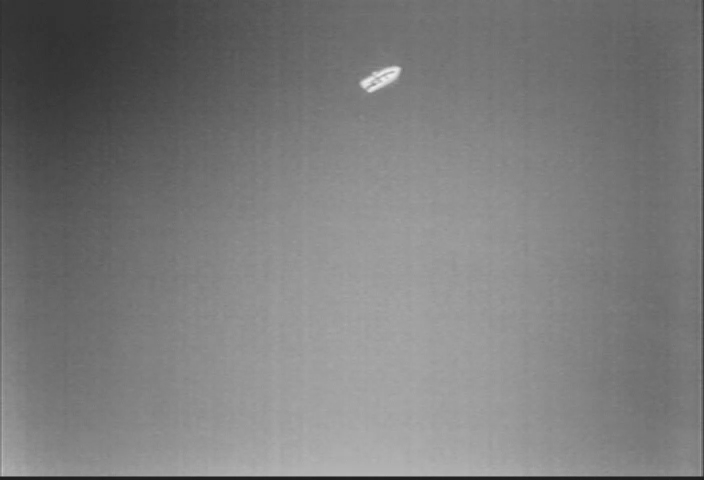
\includegraphics[width=\textwidth]{assignment_1/rapport/figures/fig1}
		\caption{caption..}
		\label{fig:2d}
	\end{subfigure}		
	\caption{Caption for all figures}\label{fig:2}
\end{figure}

\subsection*{Problem 2.5}
The Nomoto model can be written as
\begin{equation}
	\frac{r}{\delta} (s) = \frac{K}{Ts+1}
\end{equation}
and the equations for the roll and pitch rate as
\begin{equation}
\begin{aligned}
	&\dot{p} + 2\zeta_p\omega_p p + \omega_p^2 \phi = 0\\
	&\dot{q} + 2\zeta_q\omega_q q + \omega_q^2 \theta = 0
\end{aligned}
\end{equation}

\subsection*{Problem 2.6}
References can be placed in the bibliography.bib and referred to as \cite{Fossen2011} and \cite{Fjellstad1994857}.
